\chapter{Related Work}
\label{chap:related_work}
\section{Triangulation}
Consider a source language \emph{s}, pivot language \emph{p} and target language \emph{t}. When using the \emph{cascading} approach, we build two systems, between \emph{s} and \emph{p} and between \emph{p} and \emph{t}. Given a test set in \emph{s}, it is first translated to \emph{p} and those output translations are then translated into the target language \emph{t}, making decoding twice as expensive as well. We do not report our results on using cascading for various reasons. Firstly, translating the output of a source pivot system trained and tuned on little data will lead to propogation of errors. Secondly, we will need three development sets, one for each system. Finding standard development sets for low-resource languages is unlikely. Finally, it has been shown before that cascading does not give the most fluent translations.~\cite{Utiyama:07} compared pivot-based triangulation with cascading using all of multi-parallel europarl, observing that pivot-based methods outperformed cascading.

 The second approach is the pivot-based approach where a triangulated phrase table is generated between the source and target, by using the common pivot phrases between the source pivot and pivot target tables~\cite{Utiyama:07,Cohn:07}.~\cite{Utiyama:07} observed that the triangulated table was able to achieve comparable BLEU scores to the direct system for French, German and Spanish. This could be owing to the fact that the data comprised multi-parallel 560K sentences.~\cite{Cohn:07} observe that multiple pivot languages lead to more fluent translations compared to one pivot language. Multiple pivot language lead to multiple alternative translations, thus, increasing phrase coverage and rewarding the more appropriate translations and reducing out-of-vocabulary words further. They also propose a systematic way of combining the triangulated translation model with the direct model using linear interpolation and log-linear interpolation, although they assume a uniform weight for both the models. To ``simulate'' a low-resource scenario, the top 10K multi-parallel sentences are considered for source pivot, pivot target and source target systems. As we will observe later, real low-resource scenarios are significantly different from how it was simulated in~\cite{Cohn:07}.~\cite{Nakov:12} propose a language-independent approach to improving translation for low-resource languages, but the approach assumes the presence of a resource-rich language that bears similarity to the low-resource language, the similarities helping in creating a large triangulated phrase table. In~\cite{Nakovemnlp:12}, the resource-rich language is adapted to be more like the resource-poor one. Notice that this also assumes both are very similar. Results are reported using both Malay-Indonesian and Bulgarian-Macedonian, the third language being English in both cases.~\cite{Gispert:06} translate Catalan to Spanish via English by using news corpora on both source pivot and pivot target side.~\cite{Huck:12} report on BLEU score improvements by using $10^9$ parallel sentence between German and French.

 
 A common thread that binds the previous work using the approach of Triangulation is the usage of resource-rich languages. The fundamental reason behind the effectiveness of Triangulation is the reduction in the number of OOVs when using the pivot language(s). This can be observed in various forms. If the source and pivot language have a healthy vocabulary overlap, the SMT system between source-pivot is large, thus, improving translations. This factor also helps when the amount of parallel text between source-pivot is relatively low, e.g, Indonesian-English.  All the europarl languages are based on parlimentary proceedings and have minimal noise. Hence, the improvements using triangulation over the direct systems cannot be generalized for systems for low-resource languages. All the papers that use triangulation in machine translation cite either~\cite{Utiyama:07} or~\cite{Cohn:07}, both published in 2007 (and sometimes cite both of them but use either one model or the other). However, these two papers introduce triangulation for phrase-based SMT in very different ways and their models are different from each other. ``Simulating'' low-resource scenarios is ineffective in various ways. Firstly, real low-resource languages are noisy, not perfectly sentence aligned, and do not have a lot of data in the target domain. Secondly, triangulation is highly dependent on how good is the source pivot bitext. If the size of source pivot bitext is comparable to the source target, and/or is in the same domain, this increases bias in triangulation by introducting several common phrases, and, this is also not seen in a real low-resource setting.

 \alert{cite Hal} proposed domain adaptation by straight-forward duplication of features.~\cite{Bertoldi:08} suggested using alternative decoding paths when having different translation models. In our experiments, we found that alternative decoding paths did not work so well. This could be partly be because there are not that many alternatives when having two translation models of very different sizes and from different domains. When we do have alternative paths, they may not always be useful. Making trade-offs is a constant theme especially when facing low-resource languages. We want to maximize the good influence from the out-of-domain parlimentary proceedings but we do not want to undervalue translations that we get right already.~\cite{Cohn:07} propose uniform linear interpolation and log-linear interpolation. Before interpolating, they compute the joint probability of phrase pairs and use the resulting conditionals in place of the scores computed above in equations ~\eqref{eq:first} to ~\eqref{eq:last}.


 To our knowledge, before this dissertation, there has been no in-depth study of the different choices in building an SMT system using triangulation. Cascading and pivot-based triangulation have been compared~\cite{Utiyama:07,Gispert:06}, and a hybrid method has also been proposed~\cite{Wu:09} but results on using just pivot-based triangulation with real low-resource languages and comparing the different choices one needs to make has not been studied before. 
\subsection{Europarl}
Europarl is short for European Parliament and refers to the multi-parallel corpora generated by translating the proceedings of European parliament into several languages. Version 7 of Europarl now has 20 languages, from French to Estonian and Finnish. Release of the Europarl corpus led to a surge in research into more and more data-driven methods to enable Statistical Machine Translation. The results were easily reproducible and the data is very clean and sentence-aligned. Each language has development and test sets which are used to report and reproduce results. 

What does multi-parallel imply? Consider english as the common target language. A multi-parallel corpora between 20 European languages and English comprises sentences in 20 european languages which translate to the same english sentence. In Table~\ref{table:mparallel}, an english sentence and its corresponding translations in French, Spanish and German are shown. These are the 10th sentence in each of the files. The German, French and Spanish sentences are the same English sentence. When using triangulation for a multi-parallel corpora like Europarl, one is effectively tracing different steps to the same target. This helps in expanding the resulting phrase table due to many common phrases. 

\begin{table*}
	\small
	\centering
	\small
	\begin{tabular}{lr}
\toprule
Language & sentence \\
\toprule
en & i would like to ask what ideas have been developed in this report . \\
de & ich möchte fragen , welche vorstellungen man in diesem bereich entwickelt hat . \\
es & quiero preguntar qué ideas se han desarrollado en este contexto . \\
fr & je voudrais demander quelles proposition on a mis au point dans ce domaine . \\
\bottomrule
\end{tabular}
	\caption{Multi-parallel example: en = English, de = German, fr = French, es = Spanish}
	\label{table:mparallel}
\end{table*}

To give some perspective, we will discuss some results using triangulation for Europarl in this section.~\cite{Utiyama:07} used 560K multi-parallel sentences for their source pivot, pivot target and source target systems.~\cite{Cohn:07} reported results using all 700K sentences and using 10K sentences each. It is but obvious that using all the available multi-parallel sentences for triangulation leads to results that cannot be generalized to a low-resource scenario. But, consider the setting of 10K each. Considering the top 10k sentences would mean that we have a low-resource source language with which we are using a low-resource pivot language too. Even though its likely to deal with a low-resource language pair, its ineffective to use triangulation by also assuming that the pivot language itself is low-resource. Moreover, we are not effectively using the knowledge we have on using large-resource languages like French and Spanish. Using a manually set poor europarl language also necessitates the usage of multiple pivot languages to resolve OOVs, something that~\cite{Cohn:07} found effective when using triangulation. We believe that considering the top 10K sentences does not fully mimic a low-resource scenario. 

In the experiments below, we consider a constrained data setting similar to what we faced with Haitian Kreyol and Malagasy. The distribution of data is shown in Table~\ref{table:eparlsetting}

\begin{table*}
	\small
	\centering
	\begin{tabular}{lr}
		\toprule
		System & \#sentences \\
		\toprule
		direct & 100K \\
		src pivot & 50K \\
		pivot target & 2M \\
		\bottomrule
	\end{tabular}
	\caption{Our own data setting for Europarl triangulation}
	\label{table:eparlsetting}
\end{table*}

We consider top 100K sentences for our direct system while considering only top 50K of those for our source pivot system. This gives us some common words to use for triangulation but not all of 100K, which would have brought us on or above par with our direct system. On the other hand, we use all available data on our pivot target system, which is approximately 2 million lines of parlimentary proceedings of Europarl version 7. We report results on 3 languages, French(fr), Spanish(es) and German(de), all translating into English. All the results are using one pivot language. The language model used is a 5-gram Kneser-Ney interpolated language model using the English side of Europarl. 




\subsection{Results}
	The baseline models are trained on the top 100K sentences of fr-en, es-en and de-en. The results are as shown in Table~\ref{table:eparlbaselines}
\begin{table*}
	\begin{tabular}{lr}

	\toprule
	System & BLEU \\
	\toprule
	es-en & 23.32 \\
	fr-en & 19.53 \\
	de-en & 15.60 \\
	\bottomrule
	\end{tabular}
	\centering
	\small
	\caption{Baselines for our setting for all three languages}
	\label{table:eparlbaselines}
\end{table*}

	Before we report our results on Interpolation, lets find how far we can reach in terms of BLEU scores when only using the triangulated table. As the triangulated table uses multi-parallel corpora, intuitively, we should perform as well as the baseline at the least. Observe the results in~\ref{table:eparltopn}
	\begin{table*}
	\begin{tabular}{lrrrrrrr}
		\toprule
		src-tgt & pivot & baseline & top20 & top40 & top60 & top80 & top100 \\
		\toprule
		de-en & fr & \emph{15.60} & 13.32 & 13.33 & 13.35 & 13.42 & 13.03 \\
		de-en & es & \emph{15.60} & 13.37 & 13.17 & 13.49 & 13.34 & 13.36 \\
		fr-en & de & \emph{19.53} & 16.21 & 15.82 & 15.89 & 16.08 & 15.95 \\
		fr-en & es & \emph{19.53} & 17.77 & 18.15 & 17.99 & 18.01 & 18.27 \\
		es-en & fr & \emph{23.32} & 21.35 & 21.18 & 20.83 & 21.01 & 21.45\\
		es-en & de & \emph{23.32} & 18.36 & 19.19 & 19.35 & 19.23 & 18.97 \\
		\bottomrule
		\end{tabular}
		\centering 
		\small
		\label{table:eparltopn}
	\end{table*}

	But, we observe a consistent drop in BLEU scores compared to the baseline. Our constrained source pivot means that the number of OOVs for the triangulated table are more than the OOVs for the direct system. With more OOVs, the BLEU score reduces due to the reduction in the modified unigram precision as discussed in~\nameref{sec:generic_pipeline}. 

	\begin{tabular}{llrrrrrr}
	\toprule
	src-tgt & pivot & baseline & top20 & strength & M1 & joint & all \\
	\toprule
	de-en & fr & 15.60 & 15.45 & 15.62 & 15.24 & 15.52 \\
	de-en & es & 15.60 & 15.55 & 15.55 & 15.49 & 15.61  \\
	fr-en & de & 19.53 & 19.85 & 19.85 & 19.92 & 19.76  \\
	fr-en & es & 19.53 & 19.86 & 19.90 & 20.03 & 19.66  \\
	es-en & fr & 23.32 & 23.66 & 23.66 & 23.85 & 23.70  \\
	es-en & de & 23.32 & 23.68 & 23.55 & 23.84 & 23.65  \\
	\bottomrule
	\centering
	\small
	\label{table:eparlintertopn}
	\end{tabular}

	The results using the top-20 interpolation method, top20 + strength model, Model1 substition and the Joint model are reported in Table~\ref{table:eparlintertopn}. We observe that vanilla interpolation brings the BLEU score close or a little more than the baseline for all the language pairs. We see that adding the connectivity features, Model 1 scores or the Joint feature does not make a discernible difference to the BLEU scores. In figures~\ref{figure:fr_es_en} and~\ref{figure:de_es-en}, we report multiplication factors for de-en via Spanish(es) and fr-en via Spanish(es). We see that fr-en table does not grow a lot in size using Spanish as the pivot. This could be because the fr-es source pivot table does not have many rules to use in the pivot target table. On the other hand, the de-en table shows a lot more multiplicity. Having said that, both the triangulated models do not outperform their respective baselines. In fact, they get more than 1.5 BLEU points atleast compared to the baseline models. Thus, lack of multiplicity is not a factor when dealing with Europarl data like here. 
 
	\begin{figure*}
		\small
		\centering
		\includegraphics[width=0.45\textwidth]{files/Tables/fr_es_en.eps}
		\caption{fr-en triangulated via spanish not showing  a lot of multiplicity}
		\label{figure:fr_es_en}
	\end{figure*}

	\begin{figure*}
		\small
		\centering
		\includegraphics[width=0.45\textwidth]{files/Tables/de_es_en.eps}
		\caption{de-en triangulated via Spanish showing more multiplicity}
		\label{figure:de_es-en}
	\end{figure*}

\section{Domain Adaptation}


